\documentclass{article}
\usepackage{graphicx}
\usepackage[margin=1in]{geometry} % Adjust margins as you like
\usepackage{amsmath}    % for advanced math
\usepackage{amssymb}    % for additional math symbols
\usepackage{setspace}
\usepackage{cite} 
\onehalfspacing

\begin{document}

\section{Other}
\subsection{Definition of vortex}
page 311:\\
Vortex is recognized by the streamlines that resemble a helix. But that is 
not Galilean invariant, 
so maybe a \emph{bundle of vorticity lines} is the correct topological definition.\\
More precisely, vortex is a \emph{vorticity tube} surrounded by irrotational flow,
but the boundary may not be clear in viscous flow, \\
so maybe add \emph{threshold magnitude} $|omega_0|$. But how to calculate that 
threshold quantitatively?\\
A starting point would be to say that the vortex is defined by
 \emph{flow region where the vorticity prevails over the strain rate}.\cite{wu_vorticity_2006}


\section{Equations and variable definitions}

\begin{equation}
\Pi \equiv p-(\lambda +2\mu)\vartheta
\end{equation}
where $\vartheta$ is the trace of the shear tensor $D$. 
\begin{equation}
    D=\frac{1}{2}[\nabla u+(\nabla u)^T]
     \quad\text{, with } \quad D_{ii}=\vartheta
\end{equation} 
so basically $\vartheta=\nabla\cdot u$. \cite{wu_vorticity_2006}
\\
Page 256:\\
Using spheroidal coordinates, one can express the continuity equation,\\
the energy equation, using enthalpy,\\
vorticity conservation equations.\\
Than, introducing $\Gamma=rv$ to be the same for $\omega_r \text{ and } \omega_z$ as $\psi$ is for $u \text{ and } w$. 
Using those, we can come up with solutions for inviscid flow.
\cite{wu_vorticity_2006}
\section{Pictures}
Fig.3.5 from page 74.

\begin{center}
    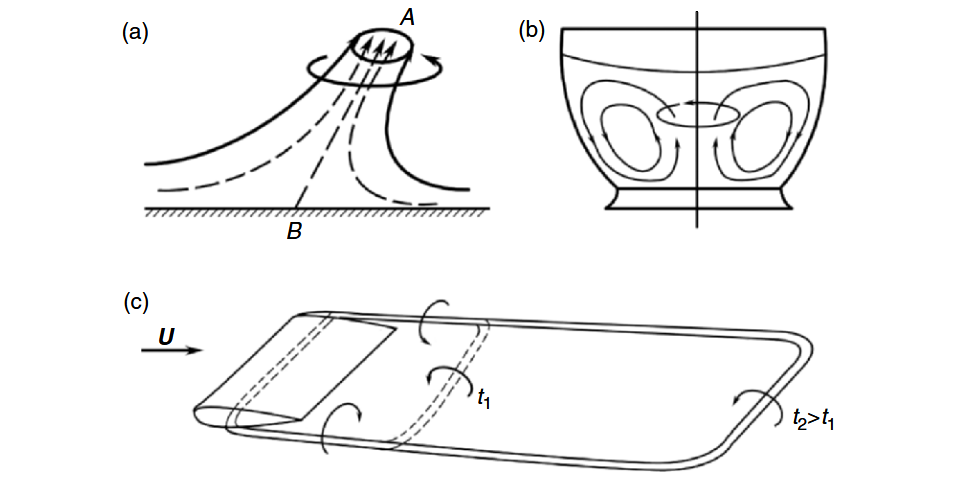
\includegraphics[width=8cm]{vorticity_lines.png}
\end{center}


\bibliographystyle{plain} 
\bibliography{MyLibrary} 


\end{document}